\chapter{Implementacja} \label{chapter:implementation}

W celu praktycznej weryfikacji koncepcji opisanych w rozdziale \ref{chapter:systemdescription} została utworzona prototypowa implementacja systemu w języku Scala, umożliwiająca utworzenie w środowisku sieciowym klastra serwerów replik, na których jako warstwa składowania danych może zostać wykorzystana dowolna lokalna baza danych typu klucz-wartość. Aplikacja jest dostępna w formie źródłowej na załączonej do pracy płycie CD --- do kompilacji przy pomocy narzędzia SBT w dowolnym systemie operacyjnym obsługującym maszynę wirtualną Javy i język Scala.

Wykorzystanie języka Scala pozwoliło na zastosowanie elementów programowania funkcyjnego w celu zachowania przejrzystości struktury projektu, która w założeniu umożliwia rozbudowę poszczególnych składników o kolejne elementy. Do komunikacji pomiędzy węzłami wykorzystana została biblioteka Akka, oparta na modelu aktorów, w którym poszczególne procesy komunikują się ze sobą wyłącznie na drodze przekazywania komunikatów --- co odpowiada uwarunkowaniom środowisk przetwarzania rozproszonego. Zwalnia to programistę z obowiązku jawnego zarządzania mechanizmami współbieżności (zamki, wątki itp.). Algorytm zapisany w postaci pseudokodu opisującego kroki wykonywane w reakcji na daną wiadomość można zapisać przy użyciu biblioteki Akka w sposób niemal bezpośredni.

Inną istotną cechą biblioteki Akka jest transparentność lokalizacji aktorów --- dla komunikujących się ze sobą aktorów nie ma znaczenia, czy są rozlokowane lokalnie, w obrębie jednej maszyny wirtualnej Javy, czy też na różnych fizycznych lokalizacjach sieciowych z komunikacją przez protokół transportowy. Odpowiednia konfiguracja środowiska pozwala na tworzenie testów integracyjnych, w których aktory tworzone są na maszynie lokalnej, podczas gdy w ustawieniu produkcyjnym są one rozmieszczone na maszynach, między którymi zestawione jest połączenie TCP.

% TODO: przypisy
% http://doc.akka.io/docs/akka/current/scala/actors.html
% http://doc.akka.io/docs/akka/current/scala/general/remoting.html

% \section{qqq} \label{section:qqq}

\section{Charakterystyka środowiska} \label{section:remarks}

System składa się z aktorów przypisanych do wielu \textit{systemów aktorów} (\texttt{ActorSystem}), z których każdy funkcjonuje w powiązaniu z określoną parą: adres IP i port TCP. Pomimo, że aktory są z punktu widzenia języka Scala niczym więcej niż obiektami, komunikacja między nimi odbywa się wyłącznie przy pomocy przekazywania komunikatów. Komunikaty wysyłane są do abstrahującej od fizycznego położenia aktora referencji typu \texttt{ActorRef} lub na określony URI reprezentujący ścieżkę do aktora (\texttt{ActorPath}) opakowany w obiekt typu \texttt{ActorSelection}. \\
Wysyłanie komunikatów, będących dowolnymi serializowanymi obiektami, odbywa się w dwojaki sposób:
\begin{itemize}
    \item Strategia \texttt{Tell} (\texttt{ref ! message}) polega na asynchronicznym przesłaniu do \texttt{ref} obiektu \texttt{message} bez oczekiwania na odpowiedź
    \item Strategia \texttt{Ask} (\texttt{ref ? message}) polega na przesłaniu do \texttt{ref} obiektu \texttt{message} w sposób synchroniczny; wywołanie \texttt{ref ? message} zwraca obiekt typu \texttt{Future}, który pozwala na deklarację oczekiwania na odpowiedź w momencie, w którym jest ona wymagana.
\end{itemize}

Każdy z aktorów w danej chwili funkcjonuje w określonym stanie (zwanym w Akka kontekstem - \texttt{context}), w którym reaguje na określone rodzaje komunikatów w odpowiedni dla tego stanu sposób. Aktor po utworzeniu swojej instancji znajduje się w początkowym stanie (kontekst zerowy) i --- jeśli zdefiniowane są inne konteksty --- podczas przetwarzania wiadomości może zdecydować o przejściu do jednego z nich. W tym przypadku, po przetworzeniu wiadomości przechodzi do nowego stanu, w którym posiada inny zbiór reakcji na przychodzące komunikaty.

Aktory przetwarzają wiadomości sekwencyjnie (w danej chwili aktor przetwarza tylko jeden komunikat), w takiej kolejności, w jakiej dostarczone są one do nich za pośrednictwem struktur \textit{skrzynek} (\texttt{Mailbox}) biblioteki Akka --- w domyślnej (użytej w implementacji) skrzynce wszystkie wiadomości posiadają równy priorytet i są przetwarzane w kolejności trafienia do niej. Użyty protokół TCP traktujemy z punktu widzenia opisu środowiska rozproszonego jako realizację abstrakcji kanałów niezawodnych, a jego dodatkową cechą jest gwarancja kolejności FIFO w obrębie jednego kanału komunikacyjnego między węzłami. Środowisko nie zapewnia innych gwarancji dotyczących kolejności przetwarzania wiadomości --- w sekcji \ref{subsection:reliablebroadcast} opisany jest zaimplementowany mechanizm rozgłaszania niezawodnego zapewniający zachowanie kolejności FIFO między węzłami.

\section{Podstawowe elementy systemu} \label{section:basicelements}

Celem utrzymania separacji zagadnień, system został podzielony na elementy odpowiedzialne za poszczególne aspekty działania systemu --- odbieranie żądań od klientów i odsyłanie im odpowiedzi, kierowanie żądań klientów do przetwarzania, proces konstrukcji wartości zgodnej z określonymi przez klienta wymaganiami oraz zarządzanie lokalnym składowaniem danych.

W tej sekcji opisane zostaną poszczególne elementy aplikacji odpowiadające wyżej wymienionym zagadnieniom, z uwzględnieniem --- tam, gdzie to istotne --- fragmentów kodu, który w pełnej wersji znajduje się na załączonej płycie CD.

\subsection{ServerEndpoint} \label{subection:serverendpoint}

Aktory typu \texttt{ServerEndpoint} są instancjonowane pojedynczo na każdym serwerze replik. Działanie tego aktora odbywa się w dwóch fazach:
\begin{itemize}
    \item Faza początkowa (kontekst zerowy) - w inicjalnym stanie aktora zestawiane jest połączenie pomiędzy serwerami replik tak, by obraz stanu klastra był spójny
    \item Faza gotowości (kontekst \texttt{ready}) - aktor przechodzi w ten stan po zestawieniu połączenia i będąc w tej fazie udostępnia interfejs do zgłaszania żądań przez klientów poprzez wiadomości:
    \begin{itemize}
        \item \texttt{GetRequest(key: String, consistency: LowLevelConsistency)} - żądanie odczytu wartości pod kluczem \texttt{key} z poziomem spójności \texttt{consistency}, określającym poziom spójności w ujęciu danocentrycznym (\texttt{SequentialConsistency}, \texttt{CausalConsistency}, \texttt{CacheConsistency}, \texttt{PRAMConsistency}).
        \item \texttt{SetRequest(key: String, value: String)} - żądanie zapisu wartości \texttt{value} pod kluczem \texttt{key}.
        \item \texttt{ClientRequest(operation: ClientOperation, w: VectorClock, client: ActorRef)} - żądanie od klienta \texttt{client} wykonania operacji \texttt{operation} z minimalnym wymaganym zegarem wektorowym \texttt{w}. Struktura \texttt{ClientOperation} zawiera unikalny dla zlecającego klienta identyfikator operacji oraz informację czy żądaną operacją jest odczyt czy zapis danych. Obsługa tego typu wiadomości dotyczy żądań klienta z zachowaniem gwarancji sesji.
    \end{itemize}

\end{itemize}
Żądania \texttt{GetRequest}, które specyfikują tylko wymagania dotyczące modeli danocentrycznych, są kierowane do powiązanego z aktorem i funkcjonującego na tej samej maszynie aktora \texttt{RequestAcceptor}, który odpowiada za koordynację procesu konstrukcji wartości z zadanymi ograniczeniami na podstawie aktualnego stanu bazy danych, a następnie odesłanie wartości do aktora \texttt{ServerEndpoint}.

Aktor \texttt{ServerEndpoint} przyjmuje także żądania w formie komunikatów \texttt{ClientRequest}, które mogą oprócz wymagań danocentrycznych zawierać oczekiwane przez klienta gwarancje sesji. % dopisać z grubsza co się z nimi dalej dzieje

\subsection{RequestHandler}

Aktory typu \texttt{RequestHandler} tworzone są każdorazowo, gdy do aktora \texttt{ServerEndpoint} nadejdzie żądanie typu \texttt{ClientRequest} - są one przypisywane do obsługi tego konkretnego żądania. Dzięki ich obecności odpowiedzialność za obsługę żądań klientów została zdjęta z aktorów \texttt{ServerEndpoint}, które powinny tylko przyjmować żądania. \texttt{RequestHandler} komunikuje się z \texttt{RequestAcceptorem} w celu zlecenia mu wykonania operacji żądanej przez klienta, po czym czeka na otrzymanie odpowiedzi. Gdy odpowiedź z \texttt{RequestAcceptora} nadejdzie, \texttt{RequestHandler} odsyła ją klientowi, a samemu kończy działanie.

\subsection{RequestAcceptor} \label{subsection:requestacceptor}

Aktory typu \texttt{RequestAcceptor} są instancjonowane pojedynczo na każdym serwerze replik jako podrzędne wobec aktora \texttt{ServerEndpoint}. Aktor ten, abstrahując całkowicie od interakcji ze środowiskiem zewnętrznym (która jest zadaniem aktora \texttt{ServerEndpoint}), odpowiada za dobór strategii konstrukcji wartości dla żądanego klucza na podstawie żądanych kryteriów spójności i za materializację w pamięci trwałej wartości dla spójności sekwencyjnej.

\subsubsection{Struktury danych} \label{subsubsection:datastructuresimpl}

Na stan tego aktora składają się następujące struktury odnoszące się do algorytmu działania systemu:
\begin{itemize}
    \item \texttt{peers} --- lista (\texttt{List[ActorPath]}) ścieżek do wszystkich aktorów \texttt{RequestAcceptor} w klastrze (oprócz samego siebie)
    \item \texttt{entropy} --- bufor entropii, entropia --- buforująca otrzymywane wiadomości jako obiekty \texttt{EntropyMessage(key, value, vectorClock, origin, demandedVectorClock)} dla każdego klucza (\texttt{Map[Key, List[EntropyMessage]]})
    \item \texttt{localVC} --- lokalny zegar wektorowy synchronizowany przy każdym odebraniu wiadomości \texttt{EntropyMessage}
    \item \texttt{lastMaterializedSeqNo} --- numer sekwencyjny (\texttt{Long}) ostatniej zmaterializowanej wiadomości
    \item \texttt{lastMaterializedCacheNo} --- numery sekwencyjne (dla spójności cache) ostatniej zmaterializowanej wiadomości dla poszczególnych kluczy (\texttt{Map[Key, Long]})
    \item \texttt{sequencedMessagesVC} --- utrzymywana w kolejności rosnących numerów sekwencyjnych
        lista otrzymanych obiektów \texttt{OrderTag} odnoszących się do wiadomości, których jeszcze
        nie można zmaterializować (zob.\ sekcja \ref{subsubsection:sequencingimpl})
    \item \texttt{VsSGrequestBuffer} --- bufor żądań, których nie udało się obsłużyć od razu po ich przybyciu do systemu ze względu na wymagane przez nie minimalne wartości lokalnego zegara wektorowego, które muszą być zachowane aby móc zrealizować dane żądanie
    \item \texttt{entropyMessagesBuffer} --- bufor wiadomości \texttt{EntropyMessage}, które nie mogły być zaaplikowane do bufora entropii ze względu na wymaganą, minimalną wartość lokalnego zegara wektorowego (\texttt{demandedVectorClock}).
\end{itemize}

\subsubsection{Dobór strategii konstrukcji wartości}

W zależności od określonego w otrzymanym żądaniu odczytu wymagania dotyczącego danocentrycznego
modelu spójności, aktor wybiera odpowiednią podklasę \texttt{ValueConstructor} (szerszy opis w
sekcji \ref{subsection:valueconstructor}), która na podstawie danego w aktualnym momencie stanu
przetwarzania (zob.\ sekcja \ref{subsubsection:datastructuresimpl}) wybierze zgodnie z algorytmem wartość dla żądanego klucza. W przypadku braku danych w entropii wartość zostanie zwrócona z pamięci trwałej (\textit{backend} --- sekcja \ref{subsection:backend}).

\subsubsection{Materializacja}

Aktor \texttt{RequestAcceptor} posiada bezpośrednią referencję do obiektu będącego podtypem klasy \texttt{KeyValueBackend}, którego interfejs jest abstrakcją fizycznego nośnika bazy danych typu klucz-wartość.

W tym nośniku składowane są wartości dla spójności sekwencyjnej, materializowane po otrzymaniu
wiadomości od procesu numerującego (zob.\ sekcja \ref{subsubsection:sequencingimpl}), podczas gdy
entropia zapisywana jest w pamięci ulotnej. Teoretycznie jednak inna implementacja systemu mogłaby
zakładać także materializację wartości dla innych poziomów spójności lub przechowywanie entropii na
wspólnym nośniku z wartościami zmaterializowanymi (np.\ w celu realizacji pewnych założeń dotyczących choćby schematu odtwarzania procesu po awarii --- ten aspekt szerzej porusza sekcja \ref{subsection:replicafailures}).

\subsubsection{Sekwencjonowanie wiadomości} \label{subsubsection:sequencingimpl}

Zgodnie z algorytmem jeden z węzłów jest wyróżniony jako sekwencer dokonujący rozstrzygania sekwencyjnej kolejności zapisów zarówno w odniesieniu do poszczególnych kluczy (dla spójności cache), jak i wspólnie dla wszystkich kluczy (dla spójności sekwencyjnej). Sekwencer rozsyła nadane zgodnie z algorytmem numery sekwencyjne opakowane w wiadomość typu \texttt{MaterializedVCOrder(orderTags: List[OrderTag])}, w której znajduje się lista znaczników wiadomości o sygnaturze \texttt{OrderTag(vectorClock, seqNo, cacheNo, key)} --- przesyłane są zatem: zegar wektorowy wiadomości, klucz danych, którego dotyczy, jej kolejność dla spójności sekwencyjnej i cache.

Warto zauważyć, że pomimo iż rozsyłając swoją decyzję o nadaniu numerów sekwencyjnych proces sekwencera zna wartość, której dotyczy dany \texttt{OrderTag}, nie jest ona przesyłana jako część tego znacznika, ponieważ jest to rola procesu, który otrzymał fizyczne żądanie wykonania zapisu. Proces otrzymujący pewien \texttt{OrderTag} i stwierdzający zgodnie z algorytmem, że jeszcze nie może dokonać materializacji wiadomości o danym zegarze wektorowym, ponieważ jeszcze nie posiada jej w swojej entropii, odłoży otrzymany \texttt{OrderTag} do późniejszego przetwarzania i powróci do niego, gdy otrzyma powiązaną z nim wartość i będzie posiadał pełen prefiks przyczynowy poprzedzający odpowiednią wiadomość.

Pomimo iż nie jest to uwzględnione w wykonanej implementacji, istnieje możliwość opóźnienia lub zmniejszenia częstotliwości rozsyłania list numerów sekwencyjnych do pozostałych procesów. Takie rozwiązanie mogłoby potencjalnie znacznie ograniczyć liczbę rozgłaszanych wiadomości, ponieważ w implementacji z rozsyłaniem sekwencji natychmiast po stwierdzeniu przez sekwencer, że może dokonać nadania numeru dla otrzymanego komunikatu, przesyłane komunikaty \texttt{MaterializedVCOrder} przenoszą pojedynczy znacznik \texttt{OrderTag}.

Sekwencer rozsyła wiadomości \texttt{MaterializedVCOrder} przy pomocy mechanizmu zgodnego rozgłaszania niezawodnego. Nierozwiązanym w prototypowej implementacji systemu problemem pozostaje kwestia awarii procesu będącego sekwencerem i przejmowania jego roli przez inny proces. Szersze rozważania na temat awarii sekwencera i możliwych sposobów na obsługę sytuacji ich występowania znajdują się w sekcji \ref{subsection:sequencerfailures}.

\subsection{KeyValueBackend} \label{subsection:backend}

% [BK] Nie powinno się stosować takich słów prosto z angielskiego bezpośrednio - może interfejs?
% [MB] Dosłowne tłumaczenie słowa "trait" to "cecha" i brzmi ono dość niezgrabnie. Nigdy więcej tego typu prac w języku polskim
Cecha \texttt{KeyValueBackend} specyfikuje interfejs dostępu do fizycznego nośnika danych przechowującego pary klucz-wartość wraz z metadanymi --- obejmującymi dla każdej przechowywanej wartości znacznik zegara wektorowego powiązany z tą wiadomością.

\begin{lstlisting}[language=Scala,caption=Definicja cechy KeyValueBackend]
trait KeyValueBackend {
  def get(key: String, consistency: LowLevelConsistency): Option[(String, Metadata)]
  def set(key: String, consistency: LowLevelConsistency, value: String,
          metadata: Metadata): Unit
  def clear: Unit
}
\end{lstlisting}

W wykonanej implementacji znajdują się dwie klasy implementujące \texttt{KeyValueBackend}: \texttt{MapBackend} wykorzystujący prostą strukturę \texttt{Map} w pamięci operacyjnej oraz \texttt{RedisBackend} korzystający z bazy danych Redis. Wykorzystanie dowolnego innego składowania danych polegałoby na utworzeniu innej klasy implementującej cechę \texttt{KeyValueBackend}, w której metody \texttt{get}, \texttt{set} i \texttt{clear} odwołują się do wybranej fizycznej bazy danych.

Konfiguracja aplikacji poprzez plik \texttt{application.conf} pozwala na określenie klas używanych w środowisku produkcyjnym i testowym w kluczach \texttt{repliflex.env.default.backend} (domyślnie \texttt{RedisBackend}) i \texttt{repliflex.env.test.backend} (domyślnie \texttt{MapBackend}).

\subsubsection{MapBackend} \label{mapbackend}

% [BK] Nie traitu, ale może interfejsu?
Najprostsza implementacja cechy \texttt{KeyValueBackend} opiera się na prostej strukturze tablicy asocjacyjnej (\texttt{Map}). Jest wygodna do stosowania w środowisku testowym --- nowe instancje obiektów \texttt{Map} są tworzone za każdym razem przy instancjonowaniu aktora \texttt{ServerEndpoint}, dzięki czemu pomiędzy testami nie ma potrzeby wykonywania operacji czyszczenia struktur. Jej zastosowanie w środowisku produkcyjnym nie jest zalecane ze względu choćby na brak trwałości przechowywania danych.

\subsubsection{RedisBackend} \label{redisbackend}

Implementacja opierająca się na bazie danych Redis wykorzystuje do dostępu do serwera bazy danych polecaną przez jej twórców bibliotekę \texttt{scala-redis} \footnote{https://github.com/debasishg/scala-redis}. Redis jest systemem bazy danych operującym w pamięci operacyjnej, posiadającym mechanizmy zrzucania zapisów do pamięci trwałej --- dzięki czemu nadaje się do zastosowania w warunkach produkcyjnych.

Redis posiada własne mechanizmy replikacji (zob.\ rozdział \ref{chapter:existingsolutions}) oparte na schemacie \textit{master-slave}, które są ortogonalne wobec rozwiązań zastosowanych w opracowanym w ramach tej pracy schemacie. Wszelkie rozważania dotyczące działania prezentowanych tutaj algorytmów zakładają brak odczytu nieświeżych danych --- po fizycznym zapisie do nośnika pary klucz-wartość, odczyt tego klucza wykonany w dowolnie krótkim czasie po zapisie zwróci wynik tego, a nie jakiegokolwiek wcześniejszego zapisu. Schemat replikacji opisany w specyfikacji Redis Cluster zapewnia, że jedynie wykonywanie odczytów bezpośrednio przez repliki \textit{slave} wiąże się z możliwością odczytu nieświeżych kopii danych \footnote{https://redis.io/topics/cluster-spec\#scaling-reads-using-slave-nodes} --- zatem przy założeniu, że odczyty odbywają się poprzez replikę \textit{master}, mechanizmy replikacji wbudowane w bazę danych Redis mogą być wykorzystywane równocześnie z zaimplementowanymi w ramach opisywanej implementacji.

Konfiguracja połączenia z serwerem Redis odbywa się w podkluczach pliku konfiguracyjnego aplikacji odpowiadających za poszczególne środowiska uruchomieniowe (\texttt{default}, \texttt{test}).

\begin{lstlisting}[caption=Konfiguracja dostępu do serwera bazy danych Redis]
repliflex {
  env {
    default {
      redis {
        host = "10.0.0.5"
        port = "6379"
      }
    }
    test {
      redis {
        host = "localhost"
        port = "6379
      }
    }
  }
}
\end{lstlisting}

\subsection{ValueConstructor} \label{subsection:valueconstructor}

Podklasy typu \texttt{ValueConstructor} odpowiadają za zbudowanie wartości dla danych wymagań dotyczących danocentrycznego modelu spójności na podstawie aktualnego stanu przetwarzania, w szczególności entropii, przechowującej dane jeszcze niezmaterializowane, i fizycznego nośnika, w którym przechowywane są wartości zmaterializowane. Wszystkie konstruktory, zgodnie z algorytmem i ze względu na specyfikę komunikacji aktorów działają w sposób nieblokujący, ograniczając się do wykonania obliczeń opartych na aktualnym stanie procesu.

Implementacja schematu konstrukcji wartości dla dowolnego innego modelu spójności polega na
utworzeniu klasy dziedziczącej z \texttt{ValueConstructor}. Jako pole \texttt{implicit} wymagany
jest każdorazowo obiekt typu \texttt{KeyValueBackend}, a także dla poszczególnych rodzajów spójności
--- w zależności od tego, jakie elementy stanu brane są pod uwagę --- inne pola posiadane przez
aktora \texttt{RequestAcceptor}, np.\ \texttt{entropy: Map[Key, List[EntropyMessage]]}.

We wszystkich przypadkach pusty bufor entropii determinuje zwrócenie wartości zmaterializowanej, spójnej sekwencyjnie, a zatem spełniająej też każdy inny rozważany model spójności.

\begin{lstlisting}[language=Scala, caption=Definicja klasy abstrakcyjnej ValueConstructor]
abstract class ValueConstructor(key: String)(implicit backend: KeyValueBackend) {
  type Value = String
  def run: Option[Value]

  protected final def getFromBackend = {
    backend.get(key, SequentialConsistency) match {
      case Some((value, _)) => Some(value)
      case _ => None
    }
  }
}
\end{lstlisting}

\subsubsection{PRAMValueConstructor} \label{subsubsection:pramvalueconstructor}

Konstruktor ten korzysta z entropii do utworzenia najświeższej wartości danego klucza spełniającej model spójności PRAM --- wymagane jest, by operacje wykonywane przez poszczególne procesy były widziane w kolejności ich inicjowania przez nie. W warunkach opisywanego systemu, w którym dostępne są kanały FIFO, wystarczy odczytać najświeższą wartość obecną w entropii dla danego klucza.

\subsubsection{CacheValueConstructor} \label{subsubsection:cachevalueconstructor}

Konstruktor w celu utworzenia najświeższej wartości danego klucza spełniającej model spójności podręcznej wykorzystuje entropię, listę znanych, ale jeszcze nie zmaterializowanych znaczników \texttt{OrderTag} oraz --- dla każdego klucza --- ostatni zmaterializowany numer sekwencyjny w obrębie tego klucza.

Algorytm opiera się na obserwacji, że istnieją scenariusze przetwarzania, w których pomimo braku ciągłości globalnych numerów sekwencyjnych w wiadomościach znanych przez proces, może on w danej chwili wykazywać taką ciągłość w odniesieniu do którejś ze zmiennych. W tej sytuacji następuje zwrócenie dla spójności cache wartości nowszej od zmaterializowanej.

\subsubsection{CausalValueConstructor} \label{subsubsection:causalvalueconstructor}

Konstruktor dla spójności przyczynowej odwołuje się do entropii oraz wartości zegara wektorowego ostatniego zmaterializowanego zapisu dla danego klucza. Zgodnie z algorytmem, począwszy od tej wartości, rekurencyjnie wyszukiwane są kolejne wiadomości, które spełniają warunki spójności przyczynowej i zwracana jest najświeższa z nich.

\subsubsection{SequentialValueConstructor} \label{subsubsection:sequentialvalueconstructor}

Najprostszy z konstruktorów tworzący wartość dla spójności sekwencyjnej ogranicza się do zwrócenia aktualnej wartości zmaterializowanej dla danego klucza --- poprzez prosty dostęp do obiektu \texttt{KeyValueBackend}.

\subsection{Client} \label{subsection:client}

Do wysyłania żądań do systemu (ściślej rzecz biorąc - do aktora \texttt{ServerEndpoint}) proponowany system wykorzystuje aktora typu \texttt{client.Base}. Aktor ten na podstawie żądań podawanych przez użytkownika na wejściu, zgodnie z określonym formatem opisanym w sekcji \ref{subsubsection:console_interface} niniejszej pracy, konstruuje obiekt typu \texttt{ClientRequest}, który jest następnie wysyłany do aktora \texttt{ServerEndpoint}, stanowiącego reprezentację serwera systemu, widoczną na zewnątrz. Serwer, poprzez aktora \texttt{ServerEndpoint} deleguje dalsze przetwarzanie do aktora \texttt{RequestHandler}, utworzonego przez niego specjalnie na potrzeby obsługi żądania. Następnie aktor \texttt{RequestHandler} komunikuje się z aktorem \texttt{RequestAcceptor} (znajdującym się ciągle na tym samym węźle systemu), zlecając mu wykonanie operacji żądanej przez klienta. Operacja może zostać wykonana natychmiastowo albo dopiero po upłynięciu skończonego, lecz nieznanego z góry czasu ze względu na niemożliwość natychmiastowego spełnienia wyspecyfikowanych w żądaniu wymagań odnośnie gwarancji sesji. W ogólności więc odpowiedź od aktora \texttt{RequestAcceptor} do \texttt{RequestHandler} następuje w sposób asynchroniczny. Gdy aktor \texttt{RequestHandler} otrzyma odpowiedź z potwierdzeniem wykonania operacji przez \texttt{RequestAcceptora}, zwraca otrzymaną odpowiedź bezpośrednio do klienta (aktora klasy \texttt{client.Base}), po czym kończy swoje działanie. Powyższy opis został zobrazowany na rysunku \ref{figure:implementation_messages_flow}.

\begin{figure}[h!]
    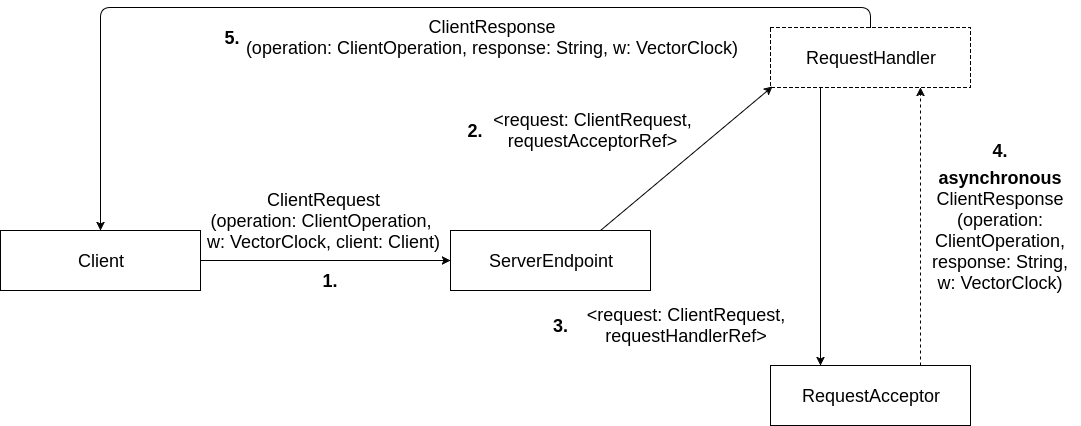
\includegraphics[width=\linewidth]{images/05-messages_flow.png}
    \caption{Schemat przepływu komunikatów w przypadku realizacji żądania klienta}
    \label{figure:implementation_messages_flow}
\end{figure}

\section{Tolerancja awarii} \label{section:faulttolerance}

W ramach prototypowej implementacji wykonanej w ramach tej pracy przygotowane i przetestowane zostały przede wszystkim stanowiące główny element algorytmu mechanizmy kontroli spójności danych dla modeli dano- i klientocentrycznych. Implementacja systemu gotowego do działania w waruknach produkcyjnych wymaga jednak podjęcia dodatkowych działań w kierunku zapewnienia odporności systemu na awarie. W niniejszej sekcji przedstawiony zostanie zarys podstawowych klas sytuacji awaryjnych jakie mogą zaistnieć w systemie, wraz z szeregiem wskazówek dotyczących możliwości rozwoju systemu w tym zakresie. 

\subsection*{Niezawodność komunikacji}

Model opisany w rozdziale \ref{chapter:systemdescription} zakłada funkcjonowanie systemu w warunkach, w których kanały komunikacyjne pomiędzy procesami, reprezentowane przez połączenia protokołu TCP, realizują abstrakcję kanałów niezawodnych, w których każda wysłana wiadomość jest w końcu dostarczona do jej adresata. Ten protokół transportowy udostępnia na bazie protokołu IP warstwy sieciowej, charakteryzującego się brakiem gwarancji dostarczenia komunikatów i zachowania ich kolejności, usługę niezawodnego transferu danych, w którym gwarantowane jest, że czytany przez proces odbiorcy strumień danych jest identyczny z tym, który był wysłany przez nadawcę.

% przypis do powyższego: http://www.bau.edu.jo/UserPortal/UserProfile/PostsAttach/10617_1870_1.pdf str. 242

Założenie o niezawodności kanałów eliminuje z rozważań możliwość występowania podziałów sieci, w
których pewna jej część składająca się z jednego lub wielu węzłów traci możliwość komunikacji z
pozostałymi węzłami. Traci w tej sytuacji istotność twierdzenie CAP omówione w sekcji
\ref{captheorem}, mówiące o nieodłączności pewnego kompromisu pomiędzy spójnością danych a
dostępnością systemu w sytuacji istnienia podziałów sieci. W przypadku jednak problemów związanych z
funkcjonowaniem innych warstw stosu protokołów sieciowych --- np.\ fizycznych awarii łącz danych --- mogą istnieć okresy, w których w systemie pomimo zachowania poprawnej semantyki przetwarzania przez proces aplikacyjny, może dochodzić do podziałów sieci. Biorąc pod uwagę taki scenariusz, należy powrócić do rozważania zachowania systemu w sytuacji wystąpienia takich awarii.

W sytuacji, gdy w systemie funkcjonuje partycja oderwana komunikacyjnie od pozostałej części systemu, rozgłoszenia zleceń zapisu pomiędzy replikami nie są w stanie przekroczyć granicy partycji. Rozważmy podział, w którym w sieci występują dwie partycje --- zatem w jednej znich znajduje się proces sekwencera. Funkcjonowanie tej partycji przyczynia się w takim układzie do utraty możliwości odzyskania przez procesy z drugiej części sieci pełnego obrazu zapisów, do których doszło w trakcie istnienia podziału, ponieważ procesy będące częścią partycji sekwencera odbiorą w krótkim czasie numery sekwencyjne wiadomości i dokonają materializacji, zrzucając odpowiednie dane ze swoich entropii. Druga z partycji będzie w tym czasie odbierać tylko zlecenia zapisów i odczytów przeprowadzane przez znajdujące się w niej procesy. Nie będą docierać do niej numery sekwencyjne wiadomości, a zatem dla spójności sekwencyjnej i podręcznej zwracane będą dane przestarzałe; w przypadku odczytów w trybie spójności przyczynowej sam brak informacji o zdarzeniach w drugiej partycji nie pociąga za sobą tak poważnych konsekwencji (pomijając fakt utraty potencjalnej możliwości pobrania z partycji sekwencera danych o zdarzeniach ze względu na ucięcie entropii) ze względu na niezależność zdarzeń.

Dostępność nierealizowalnego w praktyce w systemach asynchronicznych mechanizmu wykrycia istnienia
podziału sieci pozwoliłaby procesom znajdującym się w partycji sekwencera na natychmiastowe
zaprzestanie usuwania danych z entropii w przypadku wykrycia podziału sieci, a następnie po
stwierdzeniu ponownego poprawnego funkcjonowania systemu na przyrostową resynchronizację danych (w
rozwiązaniu o schemacie np.\ zbliżonym do stosowanego w systemie Redis, zob.\ sekcja
\ref{redisrepl}). W praktyce w celu rozwiązania problemu należałoby poszukiwać innych rozwiązań,
np.\ sięgając do mechanizmów potwierdzeń opartych na kworum.

\subsection{Mechanizmy rozgłaszania niezawodnego} \label{subsection:reliablebroadcast}

% [BK] to nie Uniform, tylko Regular c'nie?
% [MB] tak
Mechanizm rozgłaszania niezawodnego obecny w systemie, wykorzystywany do rozsyłania przez sekwencer numerów sekwencyjnych wiadomości oraz rozgłaszania zapisów przeprowadzanych przez węzły do pozostałych replik, implementuje schemat zgodnego rozgłaszania niezawodnego (\textit{Regular Reliable Broadcast}), który zapewnia otrzymanie przez wszystkie poprawne procesy wiadomości odebranej przez jeden poprawny proces. Pozwala to wyeliminować z rozważań sytuacje awarii sieci, które nie powodują utraty przez sieć systemu własności grafu spójnego, jak również awarie procesów, które nie zdołały samodzielnie rozgłosić wysyłanego komunikatu do wszystkich innych węzłów.

Rozgłaszane wiadomości \texttt{EntropyMessage} (zlecenia zapisów) i \texttt{MaterializedVCOrder} (znaczniki numerów sekwencyjnych), dziedziczące z klasy \texttt{Arriving}, są przechwytywane przez należący do aktora \texttt{RequestAcceptor} aktor \texttt{Proxy}, który następnie przekazuje je aktorowi \texttt{FIFO\_RRB\_Proxy}, który obsługuje opisany w rozdziale \ref{chapter:systemdescription} schemat rozgłaszania z wykorzystaniem wiadomości potwierdzających pozostanie procesu rozgłaszającego w stanie poprawności. Rozsyłany komunikat \texttt{message} opakowany jako \texttt{Sent(message)} jest wysyłany do należących do wszystkich węzłów aktorów \texttt{Proxy}, a dalej \texttt{FIFO\_RRB\_Proxy}, które przekazują wiadomość aktorowi \texttt{RequestAcceptor}. Dalej podąża komunikat \texttt{StayingAlive} służący jako informacja, że proces odbierający go po oryginalnym rozsyłanym komunikacie nie musi dokonywać retransmisji. W przypadku nieodebrania w pewnym czasie komunikatu \texttt{StayingAlive} następuje retransmisja wiadomości opakowanej jako \texttt{Resent(message)}.


\subsection{Awarie węzłów replik} \label{subsection:replicafailures}

Klient zlecający wykonanie operacji zapisu na danej replice nie otrzymuje od niej żadnego potwierdzenia wskazującego na powodzenie operacji i niejawnie zakłada, że operacja powiodła się. Replika, przez którą przeprowadzany jest zapis, używa opisanego w sekcji \ref{subsection:reliablebroadcast} mechanizmu rozgłaszania, który zapewnia, że do pomyślności zapisu wystarczy odebranie wiadomości przez jeden poprawny proces. Może jednak dojść do sytuacji, w której replika po otrzymaniu zlecenia ulegnie awarii, zanim wyśle wiadomość jakiemukolwiek innemu procesowi. W tej sytuacji zapis zostanie bezpowrotnie utracony pomimo, że klient zakładał, że zapis zakończył się powodzeniem.

Możliwe jest rozbudowanie implementacji o schemat detekcji sytuacji awaryjnych oparty na
potwierdzeniach odbioru zapisu wysyłanych klientowi przez repliki. Każda replika odbierająca
wiadomość \texttt{EntropyMessage}, oznaczoną dodatkowo referencją do klienta, wysyłałaby w takim
układzie do niego potwierdzenie jej otrzymania. Klient po wykonaniu zlecenia mógłby kontynuować
przetwarzanie, oczekując w tle przez określony czas na choć jedno (bazując na własnościach zgodnego
rozgłaszania niezawodnego) potwierdzenie dotyczące każdego z wykonanych zapisów. Brak potwierdzenia
w określonym czasie skutkowałby interpretowalnym w dowolny (specyficzny dla aplikacji sposób)
komunikatem o tym, że dany zapis mógł zostać zakończony niepowodzeniem. Aplikacja kliencka mogłaby
też po zleceniu zapisu blokować się do czasu otrzymania takiego potwierdzenia, co wzmocniłoby jej
pewność faktycznego wykonania operacji. Interesujące z punktu widzenia możliwości dopasowania
działania systemu do konkretnych potrzeb wydaje się udostępnienie możliwości wymuszenia wykonania
konkretnego zapisu w jednym z trzech trybów --- bez potwierdzeń, z potwierdzeniami w tle lub z
potwierdzeniami synchronizującymi. Aplikacja mogłaby wtedy np.\ wykonywać operacje krytyczne z jej punktu widzenia w trybie z potwierdzeniami synchronizującymi, a inne w trybie z potwierdzeniami w tle, mając wypracowany pewien schemat postępowania w sytuacjach, w których informacja o możliwym niepowodzeniu zapisu odbierana jest z opóźnieniem, a w międzyczasie mogły być zlecane inne zapisy.

Taki mechanizm potwierdzeń powiększyłby złożoność komunikacyjną w systemie zawierającym $n$ węzłów o $n$ wiadomości potwierdzających, nie zwiększając rzędu złożoności.

\subsection{Awarie sekwencera} \label{subsection:sequencerfailures}

Sekwencer jest newralgicznym punktem systemu ze względu na stwarzanie w przetwarzaniu pewnego stopnia scentralizowania. Poprawne działanie systemu opiera się na poprawnym funkcjonowaniu sekwencera i jego komunikacji z pozostałymi replikami, jak również konieczności istnienia w każdym momencie w systemie dokładnie jednego procesu sekwencera.

W sytuacji, gdy zatrzymane zostaje działanie procesu sekwencera, obok rozważań z sekcji \ref{subsection:replicafailures} dotyczących dowolnej repliki, występuje analogicznie zdefiniowany problem możliwości nierozesłania numeru sekwencyjnego do innych replik. Opisana propozycja mechanizmu potwierdzeń mogłaby zostać uzupełniona o dodatkową wiadomość potwierdzającą od sekwencera.

Prototypowa implementacja nie zawiera mechanizmu typu \textit{failover} zapewniającego przejmowanie przez inny proces roli sekwencera w razie jego awarii. Problem zmiany procesu pełniącego rolę sekwencera w systemie jest trudny z uwagi na brak wiedzy o konkretnym momencie awarii i ograniczone możliwości wnioskowania o spowodowanych konsekwencjach.

Przy założeniu, że sekwencer może po awarii (zawieszeniu przetwarzania i komunikacji) może powrócić do funkcjonowania, mechanizm \textit{hinted handoff} w połączeniu z rejestracją w tle potwierdzeń od sekwencera pozwoliłby na identyfikację wiadomości, które mogły nie zostać poddane sekwencjonowaniu, jak również wyznaczenie innego procesu jako tymczasowo przyjmującego wiadomości przesyłane sekwencerowi, a następnie przesyłającego mu ją jako przyrostowy obraz zmian, jakie nastąpiły w trakcie zawieszenia przetwarzania.

\subsection{Klasyfikacja własności systemu}

Charakterystyka systemu jako kładącego nacisk na utrzymanie dobrze zdefiniowanych, możliwie silnych gwarancji dotyczących spójności danych, w kontekście twierdzenia PACELC predestynuje system do rozwoju w kierunku osiągnięcia własności PC w sytuacjach wystąpienia podziału sieci; natomiast w sytuacji normalnego funkcjonowania sieci system w zależności od ustawień będzie bliższy własności L (gdy nie są używane modele spójności zorientowane na klienta, system odpowiada na żądania natychmiast) lub C (gdy klient żąda spełnienia określonych gwarancji sesji, wprowadzane są dodatkowe opóźnienia w celu zapewnienia, że dane wymagania są spełnione).

\section{Weryfikacja poprawności} \label{section:correctnesstests}

W celu zapewnienia poprawności implementacji systemu i jej zgodności ze schematem opisanym w rozdziale \ref{chapter:systemdescription} do kodu źródłowego dołączono testy napisane z użyciem biblioteki ScalaTest, rozszerzonej o moduł akka-testkit umożliwiający testowanie elementów bazujących na komponentach biblioteki Akka.

Utworzone testy dziedziczą z klasy \texttt{CustomSpec} dziedziczącej z dostarczonej przez akka-testkit klasy \texttt{TestKit} (dzięki czemu testy integracyjne mają dostęp do testowego kontekstu \texttt{ActorSystem}) i zawierającej cechy dołączające do testów elementy języka wymagań definiowanego przez bibliotekę ScalaTest.

\subsection{Testy jednostkowe} \label{subsection:unittests}

Testami jednostkowymi objęte zostały elementy systemu funkcjonujące w izolacji od elementów silnie powiązanych z komponentami środowiska Akka, charakteryzujące się jasno określonymi wymaganiami dotyczącymi danych wejściowych i wartości wyjściowych. Są to przede wszystkim klasy takie, jak podtypy \texttt{ValueConstructor} czy \texttt{KeyValueBackend}, stosowane w aktorach w sposób abstrahujący od ich implementacji i skupiający się na udostępnianym przez nie wspólnym interfejsie --- tak, by zastąpienie w określonym momencie jednej klasy inną było możliwie najprostsze.

Testy klas dziedziczących z \texttt{ValueConstructor} opisują ich zachowanie w sytuacji zadanego stanu entropii oraz danych zmaterializowanych w podklasach \texttt{KeyValueBackend}, których poprawność --- w tym jednorodność --- działania jest również zweryfikowana.

\subsection{Testy integracyjne} \label{subsection:integrationtests}

Dołączone do systemu testy integracyjne mają za zadanie weryfikację poprawności działania systemu w warunkach możliwie bliskich rzeczywistym, z perspektywy wysokopoziomowej interakcji z aktorami. Przypadki testowe zostały opracowane dla przeplotów operacji zapisu i odczytu z użyciem każdego z zaimplementowanych poziomów spójności; testami integracyjnymi objęte zostało też funkcjonowanie mechanizmu zgodnego rozgłaszania niezawodnego z zachowaniem kolejności wiadomości w kanałach komunikacyjnych.

Oprócz ustawienia dla wszystkich testów funkcjonowania biblioteki Akka w trybie lokalnym (bez traktowania referencji do aktorów jako zdalne), szczególne znaczenie dla funkcjonowania testów integracyjnych ma wybór, poprzez zawartą w pliku \texttt{application.conf} konfigurację środowiska testowego, strategii pozyskiwania obiektów \texttt{ActorSelection} (defiinowanej przez podtyp klasy \texttt{Selector}) oraz składu danych (podtyp klasy \texttt{KeyValueBackend}).

Zastosowana dla środowiska testowego strategia \texttt{DelayedSelector}, w odróżnieniu od aktywnej w innych kontekstach uruchomieniowych strategii \texttt{DirectSelector} bezpośrednio pozyskującej odnoszące się do odpowiednich aktorów obiekty \texttt{ActorSelection}, zwraca odsyłacze do aktorów \texttt{DelayerProxy}, których zadaniem jest wysłanie wiadomości do właściwego aktora docelowego z pewnym, zadanym uprzednio, opóźnieniem. Umożliwia to przeprowadzenie testów z uwzględnieniem opóźnień, jakie mogą wystąpić w rzeczywistym przetwarzaniu sieciowym. Instancje aktorów \texttt{DelayerProxy} tworzone są pojedynczo (a następnie przez cały test używane ponownie) dla każdej pary aktorów reprezentującej kanał komunikacyjny, dzięki czemu zachowana jest kolejność FIFO będąca jednym z głównych założeń dotyczących komunikacji pomiędzy procesami w systemie.

\begin{lstlisting}[language=Scala,caption=Przykładowy test integracyjny wykorzystujący opóźnianie wiadomości]
class CacheConsistencySpec extends CustomSpec {
  it should "return newer values than sequential consistency if available" in {
    registerMatcherHook(entropyMessageMatcher(
      "endpoint3",
      msg => msg.value == "igrek",
      "endpoint4"
    ), 2000 millis)

    endpoints(0) ! SetRequest("x", "1")
    Thread.sleep(400)
    endpoints(2) ! SetRequest("y", "igrek")
    Thread.sleep(200)
    endpoints(0) ! SetRequest("x", "2")
    endpoints(0) ! SetRequest("x", "3")

    Thread.sleep(200)

    val future1 = endpoints(3) ? GetRequest("x", SequentialConsistency)
    val result1 = Await.result(future1, 5 seconds).asInstanceOf[GetResponse]
    result1 shouldBe(GetResponse(Some("1")))

    val future2 = endpoints(3) ? GetRequest("x", CacheConsistency)
    val result2 = Await.result(future2, 5 seconds).asInstanceOf[GetResponse]
    result2 shouldBe(GetResponse(Some("3")))
  }
}
\end{lstlisting}

Metoda \texttt{DelayerProxy.registerMatcherHook} odpowiada za rejestrację funkcji określającej, które wiadomości mają zostać dostarczone z zadanym opóźnieniem. W tym przypadku pomocnicza metoda \texttt{entropyMessageMatcher} zwraca funkcję o sygnaturze \texttt{(pA: String, m: AnyRef, pB: String) => Boolean}, która zwróci \texttt{true} dla wiadomości od \texttt{endpoint3} do \texttt{endpoint4} ustawiającej dla dowolnego klucza wartość \texttt{igrek}. Przesyłane wiadomości, dla których funkcja ta zwraca prawdę, zostaną opóźnione o 2000 milisekund. W tym teście, weryfikującym poprawność odpowiedzi na żądania \texttt{CacheConsistency}, opóźniona jest wiadomość dotycząca innego klucza niż pozostałe (\texttt{y}), której brak w stanie odpytywanego procesu uniemożliwia odesłanie którejś z późniejszych wiadomości w trybie spójności sekwencyjnej, ale nie przeszkadza w uwzględnieniu ich dla spójności cache.

Jako skład danych natomiast w środowisku testowym najlepiej nadaje się \texttt{MapBackend}, ponieważ przy każdym utworzeniu nowej testowej instancji aktora \texttt{ServerEndpoint} tworzy on nową instancję wybranego dla danego środowiska podtypu \texttt{KeyValueBackend}, dzięki czemu nie ma potrzeby czyszczenia zmaterializowanych danych pomiędzy testami.

\section{Testy efektywnościowe} \label{section:perftests}

Charakterystyka systemu obejmująca zarówno stos technologiczny (Scala, Akka z transportem TCP) i odmienny od istniejących na rynku rozwiązań model przetwarzania rozproszonego skłoniła autorów do skupienia się w zakresie testów wydajnościowych na porównaniu sposobu zachowania systemu w zależności od wybieranych ustawień dotyczących wymagań nakładanych na spójność danych.

Szczególnie interesujące z punktu widzenia użytkownika systemu cechy wydajnościowe to wpływ
generowanego obciążenia oraz nałożonych przez klientów wymagań spójności danych na przepustowość
systemu i --- szczególnie w przypadku zastosowania gwarancji sesji --- czas odpowiedzi. Innym wartym
poruszenia zagadnieniem jest stopień nieświeżości (ang.\ \textit{staleness}) danych, które system zwraca przy dużym obciążeniu i coraz silniejszych modelach spójności.

Zaprezentowane poniżej testy nie stanowią próby kompleksowej oceny efektywności systemu, lecz można śmiało uznać je za przyczynek do potencjalnej kontynuacji jego badania.

\subsection{Środowisko testowe}

Testy przeprowadzono z wykorzystaniem chmurowej infrastruktury obliczeniowej Amazon EC2, w której dla każdego scenariusza testowego rozmieszczono serwery bazy danych na pewnej liczbie instancji maszyn wirtualnych. W środowisku Amazon EC2 rozlokowane zostały także klienty zlecające odpowiednie operacje serwerom.

Chmura obliczeniowa Amazon EC2 podzielona jest na fizycznie odległe od siebie pod względem geograficznym regiony, które z kolei dzielą się na tzw. strefy dostępności (\textit{availability zones}). Każda ze stref dostępności znajduje się w oddzielnej lokalizacji fizycznej, jednak w obrębie regionu są one połączone łączami o niskich opóźnieniach \cite{ec2}. Połączenia pomiędzy serwerami znajdującymi się w jednym regionie można zatem traktować dla rozważań o efektywności systemu jako połączenia w obrębie sieci lokalnej, zaś połączenia pomiędzy różnymi regionami lepiej reprezentują komunikację w sieci rozległej.

Testy systemu przeprowadzane były w konfiguracji imitującej sieć lokalną, tj. serwery i klienty bazy danych rozlokowane w jednym regionie usługi EC2. Utworzony system prototypowy udostępnia końcówki HTTP służące do sterowania serwerami i klientami, obsługiwane przez prostą aplikację sterowniczą zarządzającą poszczególnymi instancjami serwerów i klientów.

Wszystkie testy były przeprowadzane z użyciem strategii losowego (z rozkładem równomiernym) doboru przez klienta serwera, któremu zlecane są kolejne żądania. Szczegóły dotyczące scenariuszy testowych --- takie, jak np. opis sekwencji zgłaszania żądań czy liczba uczestniczących w przetwarzaniu serwerów --- opisane są w dalszych podsekcjach.
% http://docs.aws.amazon.com/AWSEC2/latest/UserGuide/using-regions-availability-zones.html

% \subsection{Przepustowość}

% W celu porównania parametrów wydajnościowych systemu w zależności od wybranych ustawień spójności
% można zdefiniować miarę opartą na \textbf{progu nasycenia} --- granicznej wartości obciążenia
% systemu (wyrażanego np.\ w liczbie operacji zapisu przypadających na jednostkę czasu), przy której z zadaną częstością natychmiastowy (tj. odbywający się tak szybko, jak to jest możliwe, po zleceniu operacji zapisu) odczyt zapisanych danych daje wartość wcześniejszą, niż ta, której zapis zlecono bezpośrednio przed odczytem.

% \ldots

\subsection{Przepustowość systemu}

Po zleceniu zapisu wartości bez wykorzystania gwarancji sesji i, co za tym idzie, oczekiwania na wartość będącą w pewnej zależności od wcześniejszych akcji klienta, natychmiastowy (tj. odbywający się tak szybko, jak to jest możliwe, po zleceniu operacji zapisu) odczyt danych nie musi zwrócić wartości zapisanej bezpośrednio przed tym odczytem --- niemniej bywa, że jest inaczej. Wzrost obciążenia i narzutów związanych z obsługą żądań przez serwery powoduje, że odczytywanie nieświeżych (tzn. starszych niż zapisywane natychmiast przed odczytem) wartości jest częstsze.

Zbadano wpływ na ,,aktualność'' danych odczytywanych krótko po zapisie takich czynników, jak: poziom spójności, liczba uczestniczących w przetwarzaniu serwerów i czas, jaki upływa od zlecenia zapisu do zlecenia próby odczytu ze zmiennej, do której zapisywano. Klastry złożone z 3, 7 oraz 14 węzłów w ramach testu przyjmowały serie 100 par żądań (zapis numeru porządkowego żądania i odczyt ze zmiennej, do której go zapisywano); pomiędzy każdym zleceniem zapisu i następującym po nim zleceniem odczytu oczekiwano 10 milisekund, 5 milisekund lub nie oczekiwano wcale (element regulujący obciążeniem systemu). Pomiędzy każdą parą żądań oczekiwano 10 milisekund.

Punktem wyjściowym każdej instancji testowej były serwery i klient w stanie czystym. Dla każdej konfiguracji składającej się z: danej liczby serwerów, danego opóźnienia między zapisem i odczytem i danego poziomu spójności, próba została powtórzona pięciokrotnie; za każdym razem zebrano odsetek żądań, które zwróciły wynik zapisany bezpośrednio przed odpowiednim odczytem, po czym wyniki składowe zostały uśrednione (pewnych interesujących wniosków dostarcza też w niektórych przypadkach analiza rozrzutu wyników, o czym traktuje dalsza część podsekcji).

Wykresy \ref{figure:pramgraph}, \ref{figure:causgraph}, \ref{figure:cachegraph} i \ref{figure:seqgraph} obrazują wpływ trzech wymienionych czynników na opisywaną miarę aktualności odczytów.

\begin{figure}[H]
    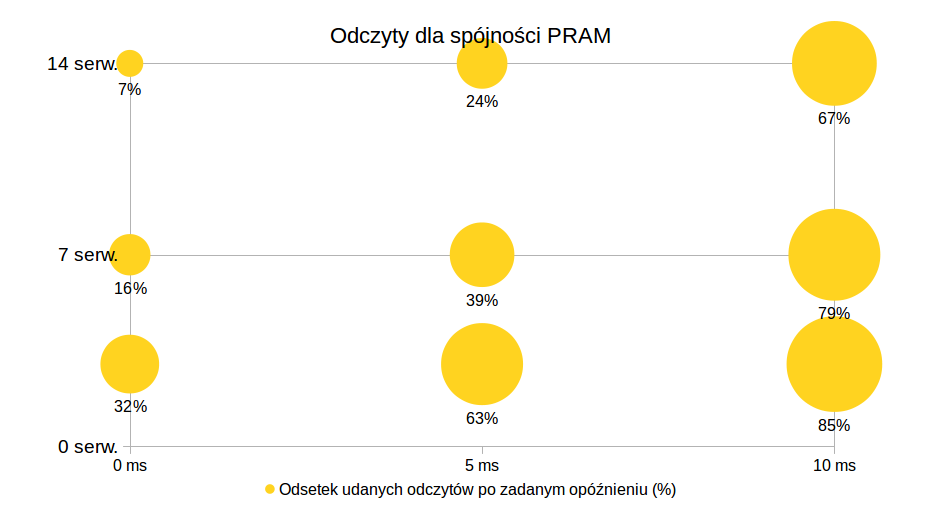
\includegraphics[width=\linewidth]{images/graphs/pram.png}
    \caption{Wykres testu powodzenia natychmiastowych odczytów dla spójności PRAM}
    \label{figure:pramgraph}
\end{figure}

Konstrukcja wartości dla spójności PRAM odbywa się z użyciem prostego algorytmu, który nie nakłada praktycznie żadnych dodatkowych ograniczeń co do spójności danych, toteż --- jak pokażą kolejne wykresy --- to właśnie odczyt ze spójnością PRAM daje największą szansę na natychmiastowy odczyt zleconego zapisu. Wpływ liczby uczestniczących w przetwarzaniu serwerów na zmniejszenie się tej szansy może być uwarunkowany faktem, że im ich więcej, tym mniejsze prawdopodobieństwo losowego wyboru serwera, do którego odpowiednio szybko dotarła zapisywana informacja.

Poszczególne próbki nie wykazywały znaczącego rozrzutu uzyskiwanych wartości, w przeciwieństwie do opisanego poniżej efektu dotyczącego spójności podręcznej i sekwencyjnej, niewidocznego w wykresach \ref{figure:cachegraph} i \ref{figure:seqgraph} zawierających dane uśrednione).

\begin{figure}[H]
    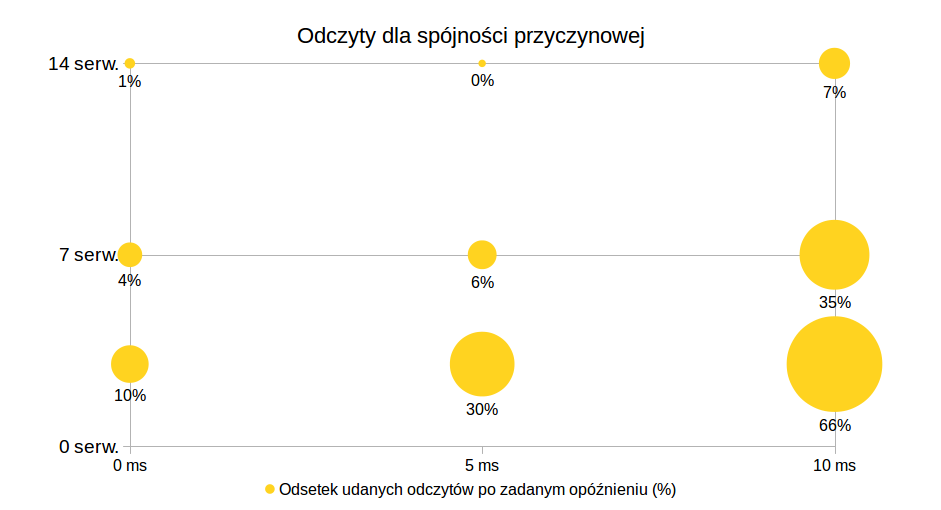
\includegraphics[width=\linewidth]{images/graphs/caus.png}
    \caption{Wykres testu powodzenia natychmiastowych odczytów dla spójności przyczynowej}
    \label{figure:causgraph}
\end{figure}

Wykonywanie testów na serwerach w stanie czystym i niewielka ilość przetwarzanych danych w każdej próbce mogłyby sugerować, że nie należy spodziewać się znaczącej różnicy w stosunku do zachowania przy spójności PRAM. Możliwe jednak, że ze względu na fakt, iż wartości dla spójności przyczynowej konstruowane są przy pomocy algorytmu wymagającego pewnego nakładu obliczeniowego, występuje zauważalne na wykresie nasilenie spadku szansy na udany natychmiastowy odczyt wraz ze wzrostem liczby serwerów lub spadkiem opóźnienia między zapisem i odczytem.

\begin{figure}[H]
    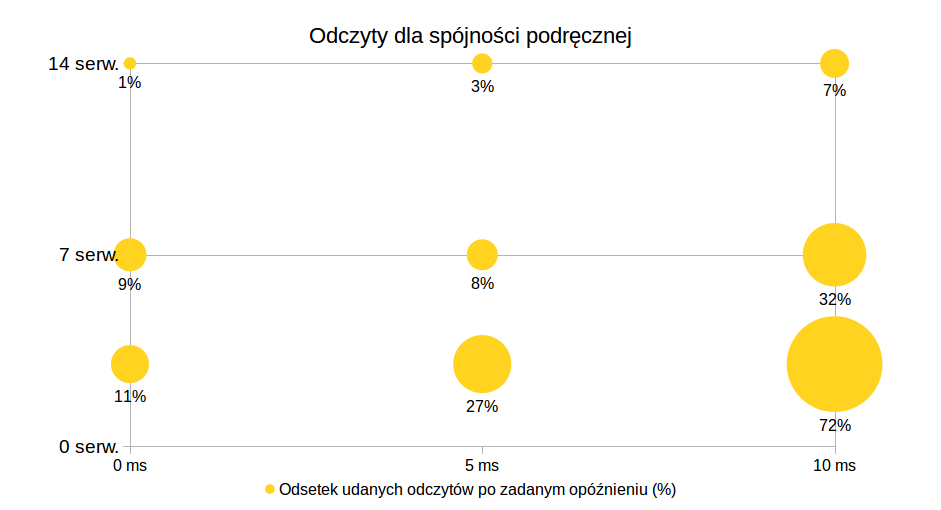
\includegraphics[width=\linewidth]{images/graphs/cache.png}
    \caption{Wykres testu powodzenia natychmiastowych odczytów dla spójności podręcznej}
    \label{figure:cachegraph}
\end{figure}

\begin{figure}[H]
    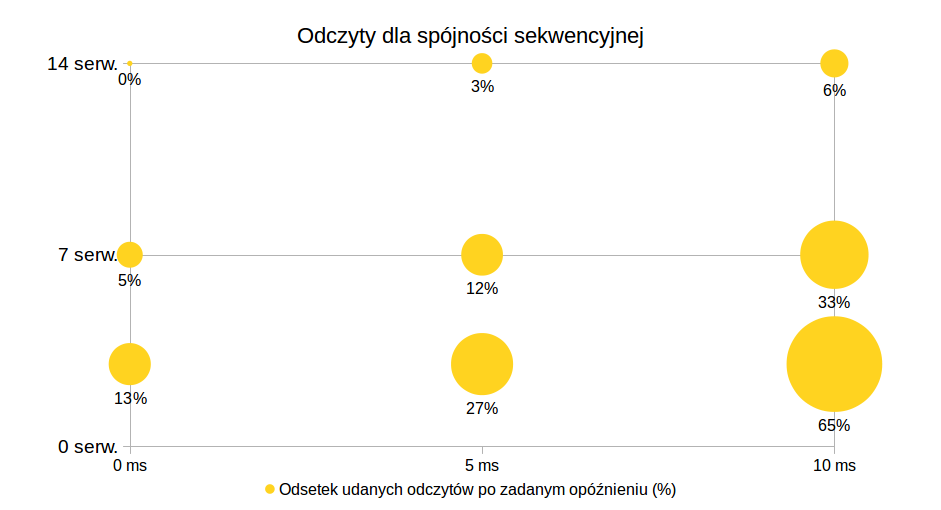
\includegraphics[width=\linewidth]{images/graphs/seq.png}
    \caption{Wykres testu powodzenia natychmiastowych odczytów dla spójności sekwencyjnej}
    \label{figure:seqgraph}
\end{figure}

Wartości dla spójności podręcznej i sekwencyjnej konstruowane są w oparciu o algorytm wykorzystywany też dla spójności przyczynowej, stąd profile wykresów \ref{figure:cachegraph} i \ref{figure:seqgraph} są zbliżone do \ref{figure:causgraph}.

Interesująca w tym przypadku jest analiza rozrzutu pomiarów dla niektórych instancji. Przykładowo, dla spójności sekwencyjnej, 7 serwerów i odstępu między zapisem i odczytem 5 milisekund, natychmiastowy odczyt powiódł się odpowiednio w: 16, 27, 6, 6 i 7 procentach przypadków; dla spójności podręcznej, 7 serwerów, bez odstępu między zapisem i odczytem pomiary wyniosły kolejno: 2, 9, 19, 13 i 0 procent.

Można przypuszczać, że konieczność transmisji przez serwer sekwencera wiadomości porządkującej zapis i odebrania tej wiadomości przez serwer, z którego klient czyta dane (co wiąże się z dodatkowym opóźnieniem transmisji) może mieć wpływ na większe zróżnicowania czasu potrzebnego na to, by serwer mógł zwrócić dany zapis jako odpowiedź na żądanie odczytu.


% \subsection{Aktualność odczytów}

% Wraz ze wzrostem obciążenia systemu żądaniami zapisu oczekiwane jest --- w sytuacji, gdy wykorzystywane są tylko wymagania danocentryczne --- odczytywanie coraz to bardziej nieaktualnych (w sensie czasu zlecenia zapisu) danych. Oprócz znalezienia progowych wartości obciążenia systemu, przy których występuje zadana częstość występowania odczytów nieaktualnych danych, potencjalnie interesujące wydaje się zmierzenie tego, w jakim stopniu są one nieaktualne, tzn. określenie o ile jednostek (mających przełożenie na rzeczywisty czas zlecenia zapisu) wcześniejsze dane --- w stosunku do ostatniego wykonanego zapisu --- są odczytywane z serwerów.

% \ldots

\subsection{Czas odpowiedzi}

W przypadku przetwarzania, w którym podłączone do klastra klienty stosują wyłącznie wymagania oparte na modelach danocentrycznych, odpowiedź jest konstruowana w sposób natychmiastowy i czas jej otrzymania zależy jedynie od występujących w sieci opóźnień i długości przetwarzania lokalnego. Czas odpowiedzi staje się istotniejszym czynnikiem do zbadania, gdy w żądaniach odczytu (i zapisu) uwzględniane są modele spójności zorientowane na klienta. Opóźnienia zależą wtedy od opóźnień propagacji danych pomiędzy poszczególnymi serwerami replik oraz od obciążenia systemu żądaniami.

Celem weryfikacji przypuszczeń na temat wpływu zastosowania gwarancji sesji na czas odpowiedzi przeprowadzono testy porównujące zachowanie obciążonego systemu w sytuacji, gdy węzły klienckie nie używają przy zlecaniu operacji gwarancji sesji, z zachowaniem przy określonym wymaganiu dotyczącym spójności zorientowanej na klienta.

Czas odpowiedzi na żądanie mierzono w milisekundach jako różnicę wskazania funkcji \texttt{System.getCurrentTimeMillis} w momencie wysłania funkcji (dołączanego do wysyłanego przez klienta do serwera obiektu \texttt{ClientRequest} i odsyłanego komunikatu \texttt{ClientResponse}) i odbioru odpowiedzi. Z uwagi na specyfikę przetwarzania wiadomości w Akka warto zaznaczyć, że dbiór odpowiedzi jest tutaj rozumiany jako moment pojawienia się jej w strukturze \texttt{Mailbox}, będącej istniejącą osobno dla każdego z aktorów kolejką, z której zgodnie z kolejnością pojawiania się w niej przychodzące wiadomości przekazywane są do funkcji \texttt{receive} aktora (co ze względu na jednoczesne przetwarzanie maksymalnie jednej wiadomości przez aktora może nastąpić z opóźnieniem).

Dla każdej z gwarancji sesji wykonano test w środowisku z pewną liczbą instancji serwerów i klientów, polegający na wykonaniu 5000 razy zdefiniowanej dla każdego ze scenariuszy rundy zleceń (w postaci opisanej w części \ref{subsubsection:console_interface}). W zależności od scenariusza, zlecenia w rundzie były identyczne dla każdego z klientów lub różniące się pomiędzy klientami, zawsze natomiast serie rund inicjowane było jednocześnie. Za wyjątkiem nielicznych zleceń wykorzystywano też synchronizację z momentem otrzymania wyniku operacji poprzez parametr \texttt{wait} w celu umożliwienia właściwego funkcjonowania mechanizmów gwarancji sesji. Wyniki zostały zebrane poprzez uśrednienie czasów odpowiedzi z 10-krotnie powtórzonego scenariusza.

\subsubsection*{Monotonic Writes}

Test czasu odpowiedzi dla gwarancji Monotonic Writes, odnoszącej się do konieczności oczekiwania przed wykonaniem kolejnego zapisu na pewnym serwerze na wykonanie się na tym serwerze wszystkich wcześniejszych operacji zapisu zleconych przez klienta (być może kierowanych do innych serwerów), został przeprowadzony dla 11 serwerów i 4 klientów. Pomiarowi podlegał średni czas odpowiedzi wszystkich żądań.

Runda zleceń w tej grupie testów miała postać:
\begin{lstlisting}
= k<n> v<n> mw wait
\end{lstlisting}
w scenariuszu aktywnej gwarancji sesji Monotonic Writes, oraz:
\begin{lstlisting}
= k<n> v<n> wait
\end{lstlisting}
w scenariuszu, w którym gwarancja ta była nieaktywna.

\subsubsection*{Read Your Writes}

Test dla gwarancji Read Your Writes, w której wymaga się, by serwer odpowiadający na żądanie odczytu miał wiedzę o wszystkich wcześniejszych wykonywanych przez klienta zapisach, przeprowadzono na 11 serwerach i 4 klientach. Wykonywano operacje odczytu i zapisu, ale wynikowa średnia czasu odpowiedzi obliczana była tylko dla operacji odczytu, oznaczonych gwarancją RYW lub bez tego wymagania.

Każda \texttt{n}-ta z kolei runda zleceń (oprócz każdej co piątej rundy) w tej grupie testów miała postać:
\begin{lstlisting}
= k<n> v<n>
\end{lstlisting}
zaś co piąta runda przyjmowała dla scenariusza z włączoną gwarancją RYW postać:
\begin{lstlisting}
= k<n> v<n> wait
? k<n> pram ryw wait
\end{lstlisting}
natomiast dla scenariusza bez gwarancji RYW:
\begin{lstlisting}
= k<n> v<n> wait
? k<n> pram wait
\end{lstlisting}
Zauważyć należy, że zgodnie ze specyfikacją specyfikatora \texttt{wait}, przed zleceniem odczytu oczekiwano tylko na jeden z wykonanych zapisów (w praktyce można byłoby to usprawnić przez dodanie specyfikatora oczekiwania na wszystkie operacje z pewnej określonej grupy). Może to mieć pewne znaczenie w kontekście funkcjonowania gwarancji sesji, ponieważ przed odczytem z gwarancją RYW nie ma gwarancji otrzymania odpowiedzi (ze znacznikami czasowymi) na wszystkie wykonane zapisy, jednak zdecydowano się na tym etapie pozostawić funkcjonowanie scenariusza w tej formie ze względu na spodziewany --- pomimo wszystko --- wpływ obecności gwarancji sesji na czasy dostępu.

\subsubsection*{Monotonic Reads}

Test dla gwarancji Monotonic Reads, której istotą jest wymaganie, by serwer odpowiadający na żądanie odczytu miał wiedzę o wszystkich wcześniejszych zapisach mających wpływ na wszystkie wcześniejsze odczyty klienta, przeprowadzono na 13 serwerach i 2 klientach. Jeden z klientów odpowiedzialny był za ciągłą aktualizację wartości w kluczu z zachowaniem gwarancji Monotonic Writes (czas odpowiedzi tych zapisów nie był brany pod uwagę). Drugi klient odczytywał wartość z użyciem włączonej lub wyłączonej gwarancji Monotonic Reads, i jego czasy odpowiedzi złożyły się na wynik końcowy.

Runda o numerze \texttt{n} dla klienta zapisującego przyjęła postać:
\begin{lstlisting}
= testkey v<n> mw wait
\end{lstlisting}
natomiast dla klienta odczytującego z gwarancją MR:
\begin{lstlisting}
= testkey v<n> pram mr wait
\end{lstlisting}
lub dla klienta odczytującego bez tej gwarancji:
\begin{lstlisting}
= testkey v<n> pram wait
\end{lstlisting}

\subsubsection*{Writes Follow Reads}

Test dla gwarancji Writes Follow Reads, której istotą jest wymaganie, by serwer odpowiadający na żądanie zapisu miał wiedzę o wszystkich wcześniejszych zapisach mających wpływ na wszystkie wcześniejsze odczyty klienta, przeprowadzono na 11 serwerach i 4 klientach. Wykonywano operacje odczytu i zapisu, ale wynikowa średnia czasu odpowiedzi obliczana była tylko dla operacji zapisu, oznaczonych gwarancją WFR lub bez tego wymagania.

Każda \texttt{n}-ta z kolei runda zleceń (oprócz każdej co piątej rundy) w tej grupie testów miała postać:
\begin{lstlisting}
? testkey pram
\end{lstlisting}
zaś co piąta runda przyjmowała dla scenariusza z włączoną gwarancją WFR postać:
\begin{lstlisting}
? testkey pram wait
= testkey v<n> wfr wait
\end{lstlisting}
natomiast dla scenariusza bez gwarancji WFR:
\begin{lstlisting}
? testkey pram wait
= testkey v<n> wait
\end{lstlisting}
przy czym obowiązują podobne uwagi dotyczące stosowania parametru \texttt{wait}, jak w przypadku gwarancji Read Your Writes.

\subsubsection*{Wyniki}

% surowe wyniki do komentarza
% 	avg
% SET(-) 5C 500R 10S	3,95
% SET(MW) 5C 5000R 10S	4,28
% 5SET(LAST SET WAITS) 1GET(-) 5C 5000R 10S (averaging gets)	2,93
% 5SET(LAST SET WAITS) 1GET(RYW) 5C 5000R 10S (averaging gets)	3,08
% GET(-) 2C 5000R 13S (writer client MW)	3,58
% GET(MR) 2C 5000R 13S (writer client MW)	3,69
% 5GET(LAST GET WAITS) 1SET(-) 5C 5000R 10S (averaging sets only)	3,73
% 5GET(LAST GET WAITS) 1SET(WFR) (averaging sets only)	3,75

Tablica \ref{latencyresults} zawiera wyniki testu przeprowadzonego według powyższego opisu.

\begin{table}[]
\centering
\caption{Wyniki testów czasu odpowiedzi dla żądań w zależności od ustawień gwarancji sesji}
\label{latencyresults}
\begin{tabular}{@{}lll@{}}
\toprule
Scenariusz testowy                   & Wymaganie gwarancji sesji & Średni czas odpowiedzi (ms) \\ \midrule
\multirow{2}{*}{Monotonic Writes}    & Nie                       & 3,95                        \\
                                     & Tak                       & 4,28                        \\ \midrule
\multirow{2}{*}{Read Your Writes}    & Nie                       & 2,93                        \\
                                     & Tak                       & 3,08                        \\ \midrule
\multirow{2}{*}{Monotonic Reads}     & Nie                       & 3,58                        \\
                                     & Tak                       & 3,69                        \\ \midrule
\multirow{2}{*}{Writes Follow Reads} & Nie                       & 3,73                        \\
                                     & Tak                       & 3,75                        \\ \bottomrule
\end{tabular}
\end{table}

Wielokrotne (10-krotne) powtórzenie testu dla każdego scenariusza i niewielkie w odniesieniu do ostatecznych wyników rozrzuty wartości próbek (tj. podobne lub mniejsze, niż różnica między wynikiem dla włączonej i wyłączonej gwarancji) pozwalają na uznanie rezultatu za zgodny z oczekiwaniami --- w warunkach obciążenia daje się zauważyć dodatkowy czas potrzebny w celu oczekiwania na pojawienie się na serwerze danych, których znaczniki czasowe będą spełniały zadane gwarancje. Jedynym niepasującym do tego obrazu elementem jest test dla gwarancji Writes Follow Reads, w którym rezultaty z włączoną i wyłączoną gwarancją WFR są podobne, a w scenariuszu z nieaktywną gwarancją notowano nieoczekiwanie większe odchylenia poszczególnych próbek; zapewne jednak przemyślana konstrukcja innego scenariusza testowego mogłaby potwierdzić wcześniejsze wnioski.

Kierunki dalszego testowania systemu pod kątem efektywności działania mechanizmu gwarancji sesji mogłyby obejmować m.in. testy przy większej liczbie instancji wraz z przeprowadzeniem prób badających zależność czasu odpowiedzi od liczby serwerów, klientów i obciążenia systemu. Interesującym zagadnieniem testowym wydaje się także sprawdzenie efektywności w sytuacjach, gdy gwarancje sesji są używane parami (tj. MR+RYW dla odczytów, MW+WFR dla zapisów).